\section{Time analysis}
First our signals are analysed in the time domain, where it is possible to see some patterns in the signals. The code used to plot the time series is the following one:
\begin{lstlisting}
[y_female,fs_female]    = audioread('female.wav');
[y_male,fs_male]        = audioread('male.wav');
[y_music,fs_music]      = audioread('music.wav');

%time domain vectors, scaled with the corresponding time period.
t_female                = 1/fs_female*(0:length(y_female)-1)';
t_male                  = 1/fs_male*(0:length(y_male)-1)';
t_music                 = 1/fs_music*(0:length(y_music)-1)';
%%
%plot of the music signal and female speech in time
figure(1)
subplot(2,1,1); plot(t_female,y_female);
ylabel('Signal amplitude'); xlabel('Time in seconds');grid;
title('Female voice signal');
subplot(2,1,2); plot(t_music,y_music);
ylabel('Signal amplitude'); xlabel('Time in seconds'); grid;
title('Music signal');

%plot of the music signal zoomed from 0.62 to 0.76 seconds
figure;
indexes_music = t_music > 0.62 & t_music < 0.76; 
plot(t_music(indexes_music),y_music(indexes_music));
ylabel('Signal amplitude'); xlabel('Time in seconds'); grid;
title('Music signal - Armonics pattern');
%plot of the female speech zoomed with voiced/unvoiced patterns

%unvoiced pattern,corresponds to s ( i shot...)
indexes_female_unvoiced = t_female > 0.17 & t_female < 0.26; 
%voiced pattern, corresponds to i ( i ...)
indexes_female_voiced = t_female > 0 & t_female < 0.9; 
figure;
subplot(211);
plot(t_female(indexes_female_unvoiced),y_female(indexes_female_unvoiced));
ylabel('Signal amplitude'); xlabel('Time in seconds');grid;
title('Female voice signal - Unvoiced pattern');
subplot(212);
plot(t_female(indexes_female_voiced),y_female(indexes_female_voiced));
ylabel('Signal amplitude'); xlabel('Time in seconds');grid;
title('Female voice signal - voiced pattern');
\end{lstlisting}
The results are shown in the following figures: \ref{fig:1},\ref{fig:2},\ref{fig:3} .\\ 
At first glance, without zooming in, both signal do not have significant patterns, but it is clear to see that the music signal is more uniform than the speech signal. \\
This is so because of the harmonic structure of the music signal: it consists of several harmonics, which are an integer multiple of the fundamental frequency.
The same can be said for some sounds in the human speech: letters like \textit{a},\textit{i},\textit{v},\textit{b}, etc... are \textit{voiced} sounds, which means that those are sounds similar to the one made by musical instruments.\\
On the other hand, letters like \textit{s},\textit{c}, \textit{f} are \textit{unvoiced} sounds. The main difference between \textit{voiced} and \textit{unvoiced} letters is that in the latter the person does not make any vocal cord vibrate: because of that we don't have an harmonic structure in \textit{unvoiced} sounds, being then a more noisy signal (it is only air passing through the larynx).\\ \\
The music signal, if we zoom in a smaller time patch, has a clear harmonic structure (it is easy to see the sinusoidal pattern), and this is shown in figure: \ref{fig:2}.\\ \\
For the female speech we can look for example at the start of the signal, where we have both a voiced and an unvoiced signal: \textit{i} and \textit{s}.
In figure \ref{fig:3} we can see in the top graph the time series of the unvoiced sound, which starts after $0.1$ seconds, and corresponds to the letter \textit{s}. In the bottom graph we have the voiced sound, which is the first letter being pronounced by the woman, \textit{i}.
\\Notice how the unvoiced signal just looks like random noise, whilst the voiced signal  has a clear harmonic structure.

\begin{figure}[h]
		\centering	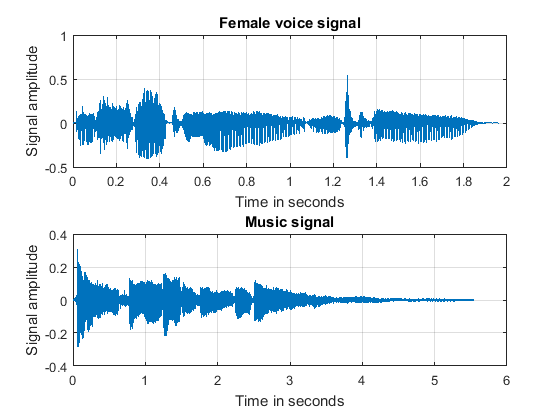
\includegraphics[width=0.77\linewidth]{./images/music_female_time.png}
		\caption{Time series of the female speech and music signal}
		\label{fig:1}	
\end{figure}

\begin{figure}[h]
\centering
\begin{minipage}{.5\textwidth}
  \centering
  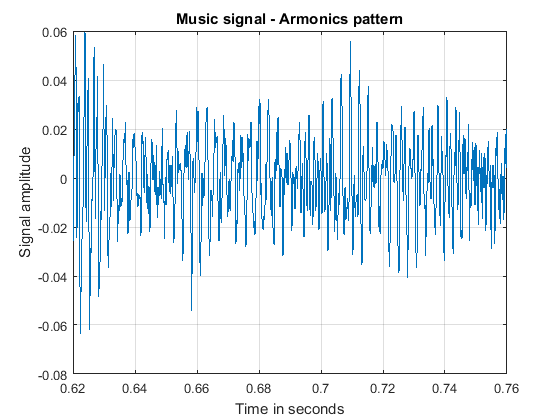
\includegraphics[width=0.95\linewidth]{./images/music_time_zoom.png}
  \captionof{figure}{Harmonic structure of the music signal}
  \label{fig:2}	
\end{minipage}%
\begin{minipage}{.5\textwidth}
  \centering
  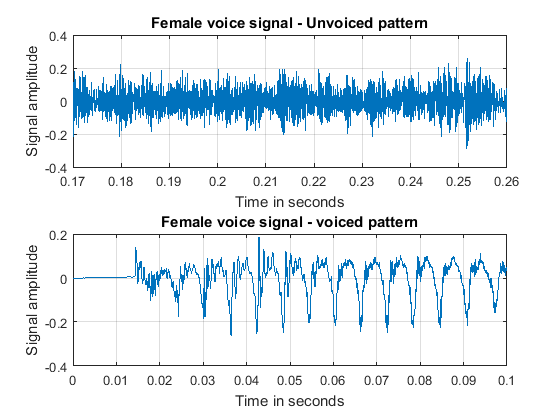
\includegraphics[width=0.95\linewidth]{./images/female_time_zoom.png}
   \captionof{figure}{Plot of unvoiced and voiced sounds of the female speech}
   \label{fig:3}	
\end{minipage}

 
\end{figure}
